\section{Method}

\begin{figure*}[t]
    \centering
    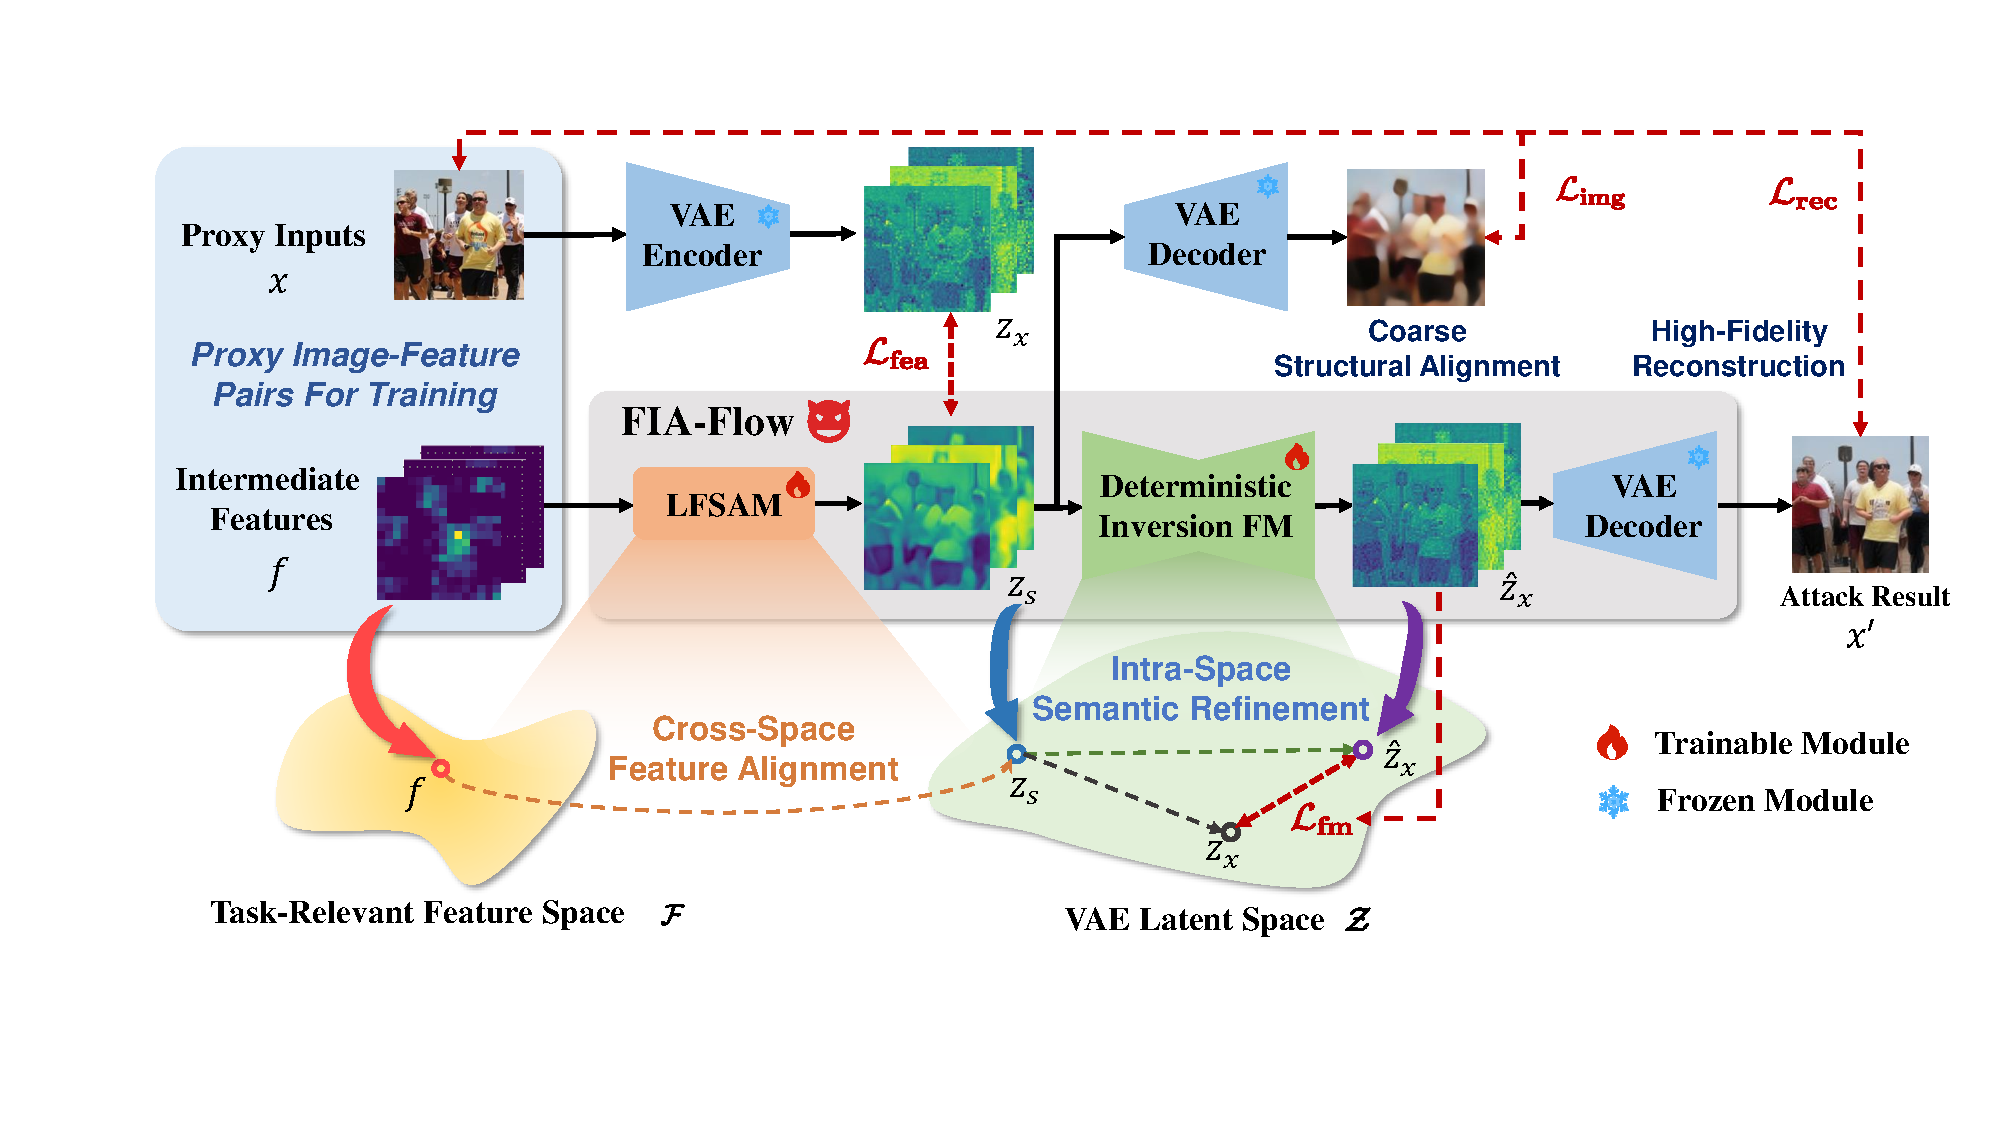
\includegraphics[width=0.9\linewidth]{img/fig-pipe-1111.pdf}
    \caption{The pipeline of FIA-Flow. The method reconstructs a private image $x$ from the corresponding intermediate features $f$. It first maps $f$ to a latent code $z_s$ by the Latent Feature Space Alignment Module, then uses the Deterministic Inversion Flow Matching module to refine it into $\hat{z}_x$. Finally, the attack image $x'$ is obtained by a pre-trained VAE decoder from $\hat{z}_x$.}
    \label{fig-pipe}
\end{figure*}
\subsection{Overview and Problem Formulation}
Let $M: \mathcal{X} \to \mathcal{F}$ denote the head submodel of the victim Split DNN system, where $\mathcal{X} \subseteq \mathbb{R}^{H \times W \times C}$ is the space of private input images. 
For a given input $x \in \mathcal{X}$, the model $M$ produces an intermediate feature $f=M(x)$ at a specific split layer, where $f \in \mathcal{F} \subseteq \mathbb{R}^{D_f}$ and $D_f$ is the feature dimension.
The primary objective of FIA is to learn an inversion mapping $G: \mathcal{F} \to \mathcal{X}$ that can reconstruct the original input $x'$ from its corresponding feature $f$, such that the reconstructed image $x' = G(f) \approx x$ is perceptually and semantically indistinguishable from the original input $x$. 

Our attack operates under a black-box assumption, where the architecture and parameters of $M$ are unknown. 
We can only query to obtain a set of image-feature pairs $\mathcal{D} = \{ (x_i, f_i) \}_{i=1}^{N}$ for training.
To achieve this, FIA-Flow adopts an alignment-refinement strategy, as shown in Fig. \ref{fig-pipe}.
We decouple the complex inversion mapping $G$ into a two-stage process: a structural alignment stage and a semantic refinement stage, which can be formulated as:
\begin{align}
x'=G(f) = \text{Dec}(G_{\text{refine}}(G_{\text{align}}(f)) )
\end{align}
$\text{Dec}:\mathcal{Z} \to \mathcal{X}$ denotes the decoder of Variational Autoencoder (VAE)  \cite{kingma2013auto}. 
The alignment stage $G_{\text{align}}: \mathcal{F} \to \mathcal{Z}$ establishes structural correspondence by aligning the task-relevant feature spaces and latent space of the VAE. 
However, this alignment primarily yields an off-manifold representation, which lacks the semantic richness.
Therefore, the refinement stage $G_{\text{refine}}: \mathcal{Z} \to \mathcal{Z}$ performs intra-space semantic enhancement, correcting the distributional mismatch to ensure high-fidelity inversion.

\subsection{Latent Feature Space Alignment Module}
\paragraph{Motivation and Objective} 
A fundamental challenge in FIA arises from the space gap between $\mathcal{F}$ and the latent space $\mathcal{Z}$. 
Since $\mathcal{F}$ is task-specific and optimized for classification rather than synthesis, its structure is inherently incompatible with the manifold of $\mathcal{Z}$ \cite{yosinski2014transferable}.
Therefore, a direct mapping from feature $f$ to image $x$ is ill-posed.
To bridge this gap, we propose the LFSAM to transform a given intermediate feature $f$ into a latent tensor $z_s=G_{\text{align}}(f)$, which is designed to be both dimensionally compatible and structurally aligned with the latent space of VAE. 
The VAE is selected for its continuity and structured latent space, offering an ideal manifold for stable and coherent refinement \cite{doersch2016tutorial}. 
Meanwhile, the low-dimensional latent space reduces the complexity of the hypothesis class, making alignment learning easier to generalize under few-sample conditions \cite{yang2024few}. 
This enables FIA-Flow to effectively learn and extrapolate robustly to unseen features.


\paragraph{Cross-Space Feature Alignment}  
LFSAM comprises a learned upsampling module, a backbone, and a Feature Aggregation Network (FAN) to synthesize a comprehensive latent representation. 
To accommodate features with varying resolutions across different network layers, we employ a PixelShuffle-based spatialization layer $PS: \mathbb{R}^{(r^2  C_{in}\times  H_{in} \times W_{in})} \to \mathbb{R}^{(C_{in} \times r  H_{in} \times r W_{in})}$. 
Unlike standard interpolation, this operation provides a learned transformation that unfolds channel-encoded spatial information into an explicit geometric grid. 

The backbone $B(\cdot)$ processes $f$ through a hierarchical encoder, which extracts a set of feature maps $\{e_1,e_2, \ldots, e_L\}$. 
Its corresponding decoder reconstructs the output progressively from the deepest feature level. 
Crucially, at each stage, the decoder integrates features from the corresponding encoder stage via skip connections, a process formulated as $d_{i+1}=\mathcal{D}(concat(d_i,e_{i}))$. 
To capture global context and long-range spatial dependencies, we embed self-attention mechanisms within the backbone layers, producing $F_{d}=B(f)$. 
Meanwhile, FAN projects each $e_i$ into a shared space via $1\times 1$ convolutions $\phi_i$ then concatenates and fuses them: $F_{fan}=\text{Conv}_{\text{fuse}}(\text{concat}_{i=1}^L(\phi_i(e_i)))$.
The final aligned feature is:
\begin{equation}
z_s = \text{Conv}_{\text{out}}(F_{d} + F_{fan}),
\end{equation}
which serves as a structural alignment feature for the subsequent refinement stage.

\subsection{Deterministic Inversion Flow Matching}
\label{sec:fm} 
\paragraph{Motivation and Objective}
With the space-aligned latent feature $z_s$ obtained from LFSAM, we aim to generate a photorealistic inversion image $x'$ that closely resembles the private input $x$. 
A naive approach involves directly decoding the aligned feature $z_s$ using a pre-trained VAE decoder $x' = \text{Dec}(z_s)$. 
However, experimental results demonstrate that this straightforward method produces suboptimal results with severe blurriness and semantic inconsistencies. 


The core issue is a distributional mismatch between the aligned features and the natural data manifold. 
Although LFSAM ensures that $z_s$ conforms to the dimensional requirements of the VAE latent space, it fails to guarantee that $z_s$ follows the same distribution as the authentic latent feature generated by the VAE encoder from natural images.
Since $z_s$ originates from a task-specific feature transformation, it likely resides in off-manifold regions of the latent space $\mathcal{Z}$. 
The VAE decoder is trained exclusively on on-manifold samples, cannot interpret out-of-distribution inputs, resulting in degraded reconstruction quality.
Therefore, we propose the DIFM to enhance semantic expressiveness based on the previous structural alignment.
\paragraph{Intra-Space Feature Enhancement}
To overcome the limitations of direct decoding, we reframe $z_s$ as a high-quality starting point for a generative process rather than a final latent feature. 
We employ the DIFM to learn a deterministic vector field $v_\theta(z,t)$ that transforms the distribution of our structurally-aligned features $p_0 = p(z_s)$ to the target data distribution $p_1 = p(z_x)$, where $z_x=\text{Enc}(x)$.
This approach adapts the standard FM framework by replacing the conventional Gaussian prior $p_0' = \mathcal{N}(0, I)$ with our meaningful initializations $p(z_s)$.


Specifically, we define a linear interpolation path between the starting point $z_s$ and its corresponding target $z_x$ as $z_t = t \cdot z_x +(1-t) \cdot z_s $ for $t\in [0,1]$. 
DIFM is trained to approximate this target field $u_t={dz_t}/{dt}=z_x-z_s$. 
Once trained, this learned vector field defines the trajectory of each point via the probability flow ordinary differential equation (ODE), $d\hat{z}_t/{dt}=v_{\theta}(\hat{z}_t,t)$, and the continuity equation describes its distributional evolution:
\begin{equation}
\partial_t p_t(z) + \nabla_z \cdot (p_t(z) v_\theta(z, t)) = 0.
\end{equation}
This equation formalizes the desired behavior of $v_\theta(z,t)$, ensuring it guides the population of points from the initial distribution $p_0$ to the target data distribution $p_1$.
Since LFSAM already produces $z_s$ close to $z_x$, the learned vector field is simple, allowing us to replace an expensive ODE solver with a single forward Euler step from $t=0$ to $t=1$:
\begin{equation}
\hat{z}_x =\hat{z}_1= z_s +v_\theta(z_s, t=0).
\end{equation}
The final inversion image $x'$ is decoded by the VAE: $x'=\text{Dec}(\hat{z}_x)$. 
By conditioning the generative process on a meaningful initialization, our strategy effectively transforms a complex generation task into a residual correction problem. 
This simplifies the learning dynamics of the vector field, reducing the data requirements, thereby enabling high-fidelity inversion even with limited training samples.



\subsection{Training Strategy}
\label{sec:training}
We adopt a two-stage training paradigm for the FIA task. This decoupled approach is designed first to establish a space alignment and then to optimize the generative model. \\
\textbf{Stage 1: Training the LFSAM.}
In the first stage, we train the LFSAM to learn a mapping from the task-relevant input features $f$ to the VAE latent space. Our objective is to ensure that the LFSAM produces structured features $z_s$ that closely approximate the ground truth (GT) VAE latent feature $z_x$ of the corresponding images $x$.
We employ a pre-trained, frozen VAE encoder to obtain target latent codes $z_x = \text{Enc}(x)$. 
To ensure feature space alignment, we minimize the L2 distance between the $z_s$ and $z_x$:
\begin{equation}
\label{eq-fea}
\mathcal{L}_{\text{fea}} = \mathbb{E}_{(x, f) \sim \mathcal{D}} \left[ \| z_s - z_x \|_2^2 \right].
\end{equation}

To enforce perceptual coherence, we apply an image-domain reconstruction loss. We decode the generated latent $z_s$, and minimize the L1 distance to the GT image $x$:
\begin{equation}
\label{eq-img}
\mathcal{L}_{\text{img}} = \mathbb{E}_{(x, f) \sim \mathcal{D}} \left[ \| \text{Dec}(z_s) - x \|_1 \right].
\end{equation}

The total loss for Stage 1 is the sum of these two losses:
\begin{equation}
\mathcal{L}_{\text{s1}} = \mathcal{L}_{\text{fea}} + \mathcal{L}_{\text{img}}.
\end{equation}
\begin{figure*}[t]
    \centering
    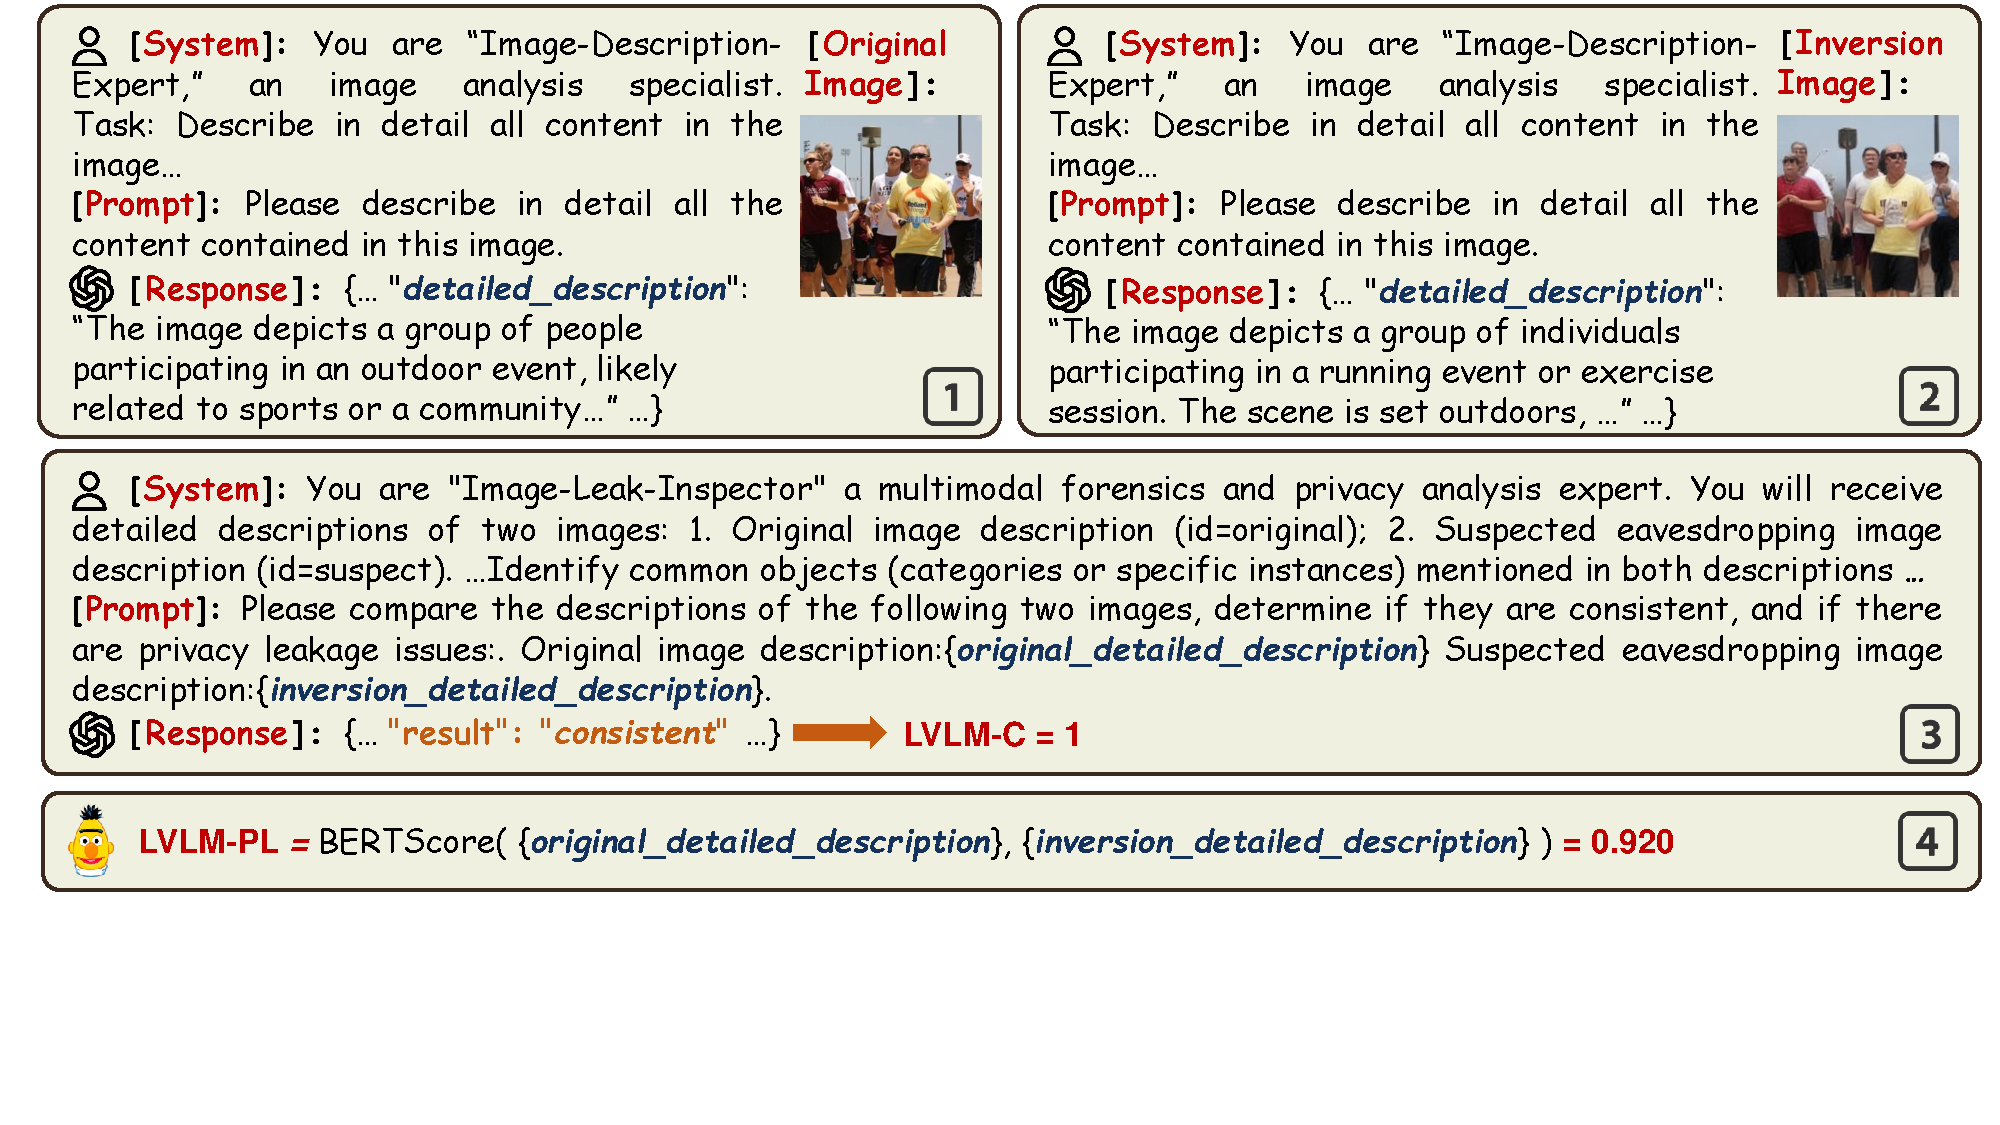
\includegraphics[width=0.95\linewidth]{img/fig4}
    \caption{An illustration of LVLM-C and LVLM-PL evaluation. \ding{172} The LVLM is prompted to describe the original image. \ding{173} The LVLM is then prompted to describe the inversion image. \ding{174} The LVLM compares these two descriptions to ascertain if the same object is identified. A consistent result yields the LVLM-C value of 1. \ding{175} LVLM-PL is obtained by computing the BERTScore \cite{zhang2019bertscore} between the two descriptions. 
    }
    \label{fig-lvlm}
\end{figure*}

Stage 1 ensures that the LFSAM learns a meaningful projection into the VAE latent space, providing a solid foundation for the subsequent stage. \\
\textbf{Stage 2: Training the DIFM.}
In the second stage, we freeze the LFSAM and train the DIFM, which takes the precomputed features $z_s$ as a starting point and learns to generate the final image $x'$. 
The training objective for this stage is a combination of two losses:

\begin{enumerate}
    \item \textbf{Flow Matching Loss ($\mathcal{L}_{\text{fm}}$):} 
    This is a regression loss that minimizes the L2 distance between the model's predicted vector field $v_\theta(z_t,t)$ and the target vector field $u_t$:
    \begin{equation}
    \mathcal{L}_{\text{fm}} = \mathbb{E}_{t \sim \mathcal{U}[0,1], (x,f) \sim \mathcal{D}} \left[ \| v_\theta(z_t,t) - u_t \|_2^2 \right].
    \end{equation}

    \item \textbf{Reconstruction Loss ($\mathcal{L}_{rec}$):} To ensure that the final output $x'$ is perceptually and semantically faithful to the original image $x$, we apply a reconstruction loss directly in the image space. 
    This loss is a combination of Learned Perceptual Image Patch Similarity (LPIPS) \cite{zhang2018unreasonable} loss and a pixel-wise L1 loss:
    \begin{equation}
    \label{eq-rec}
    \mathcal{L}_{\text{rec}} = \mathbb{E}_{(x,f) \sim \mathcal{D}} \left[\ \mathcal{L}_{\text{LPIPS}}(x', x) + \mathcal{L}_{\text{L1}}(x', x) \right].
    \end{equation}
\end{enumerate}



The final loss for Stage 2 is the sum of these two losses:
\begin{equation}
\label{eq-all}
\mathcal{L}_{\text{s2}} = \mathcal{L}_{\text{fm}} + \mathcal{L}_{\text{rec}}.
\end{equation}



